\section{Parallelization Techniques and Implementation}

\subsection{Parallelization with MPI}
To achieve scalable simulation of information and congestion propagation on large-scale smart road systems, this project employs the Message Passing Interface (MPI) to distribute the computational workload across multiple processors. Each processor (MPI rank) is responsible for evolving a subset of the overall grid representing spatial regions (e.g., states or road cells). Inter-process communication is used to exchange boundary (ghost) cells, enabling accurate interaction across adjacent regions.

MPI was selected due to the following advantages:
\begin{itemize}
    \item \textbf{Scalability}: MPI allows distributing computation across multiple cores and nodes, making it suitable for simulating large grids (e.g., 50+ cells).
    \item \textbf{Explicit communication}: As our model requires interaction between neighboring cells, MPI’s explicit control over data exchange provides both flexibility and performance.
    \item \textbf{Process isolation}: Each process handles only its assigned cells, reducing memory contention and increasing cache efficiency.
\end{itemize}

\subsubsection*{MPI Parallelization Workflow}
The main simulation procedure using MPI consists of the following steps:
\begin{enumerate}
    \item \textbf{Grid Partitioning (Rank 0)}: The global grid is first mapped using a cell ID mapping loaded from a CSV dataset. The function\\\texttt{divideIntoOptimalBlocks()} chooses the most balanced partitioning scheme. Cells are grouped into blocks and assigned to ranks.
    
    \item \textbf{Initial Communication}: Rank 0 broadcasts:
    \begin{itemize}
        \item Block-to-rank map
        \item Cell neighbor relationships
        \item Ghost neighbor relationships
    \end{itemize}
    Each rank initializes its local SIRCell grid using \texttt{setGridFromLocalData()}.

    \item \textbf{Ghost Cell Communication}: During each time step, ghost boundary cells are exchanged using non-blocking MPI operations:
    \begin{itemize}
        \item \texttt{MPI\_Isend} and \texttt{MPI\_Irecv} transfer S, I, R values to/from neighboring ranks.
        \item \texttt{MPI\_Barrier} ensures synchronization.
        \item Mapping from local index $\rightarrow$ global ID and global ID $\rightarrow$ owner rank is used to build send/receive buffers.
    \end{itemize}

    \item \textbf{Local Update}: Each cell is updated using \texttt{rk4StepWithNeighbors()}, incorporating the influence of both local and ghost neighbors. A normalization step ensures \( S + I + R = 1 \) for every cell.

    \item \textbf{Result Collection}: At the end of the simulation, each rank outputs its local average S, I, R to a time-series vector. Optionally, Rank 0 gathers global results for visualization.
\end{enumerate}

\subsection{MPI Functionality Highlights}
To understand performance behavior and potential bottlenecks, we conducted fine-grained timing analysis across different phases. Each rank logs the time spent in key MPI-related sections using a custom timing utility module\\ (\texttt{TimingUtils.cpp}). This provides rank-specific insights into load balancing and communication overhead.

\begin{table}[h]
\centering
\begin{tabular}{|l|p{9cm}|}
\hline
\textbf{Phase} & \textbf{Description} \\
\hline
\texttt{distributeBlocks()} & Initial grid partitioning on rank 0 \\
\texttt{Total\_MPI\_Prep\_In\_Loop\_RankX} & Time preparing ghost data buffers per step \\
\texttt{Total\_MPI\_Comm\_In\_Loop\_RankX} & Actual non-blocking send/receive time \\
\texttt{Total\_Local\_Computation\_RankX} & RK4 updates using local + ghost values \\
\texttt{runSimulation\_TotalWallTime} & Overall simulation time (barrier-to-barrier) \\
\hline
\end{tabular}
\caption{MPI Timing Categories}
\end{table}

We observed that computation dominates total execution time, but MPI communication becomes significant as the number of ranks increases.
\begin{figure}[!htb]
    \centering
    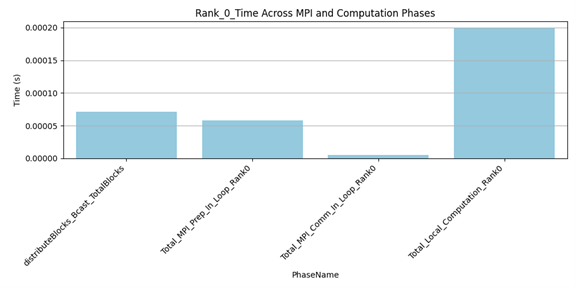
\includegraphics[width=14cm]{Images/pic1.png}
\end{figure}

\subsection{Visualization of Spatial Communication}
To explore the impact of rank-based spatial decomposition, we visualize the evolution of infection intensity per rank over time. Each MPI rank controls a specific grid region (e.g., a block of US states), and infection spreading dynamics are influenced by local conditions and ghost exchange.

Key observations:
\begin{itemize}
    \item Some ranks remain uninfected due to lack of spatial contact (e.g., isolated blocks).
    \item Peak infection times vary across ranks due to asynchronous propagation.
\end{itemize}
\begin{figure}[!htb]
    \centering
    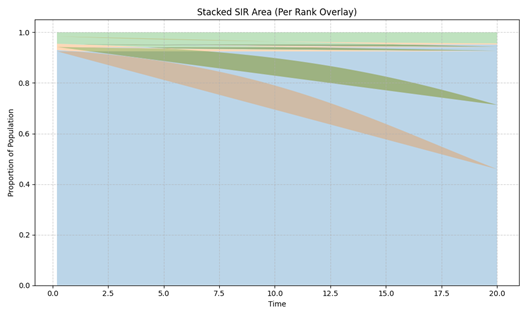
\includegraphics[width=14cm]{Images/pic3.png}
    
\end{figure}\begin{figure}[!htb]
    \centering
    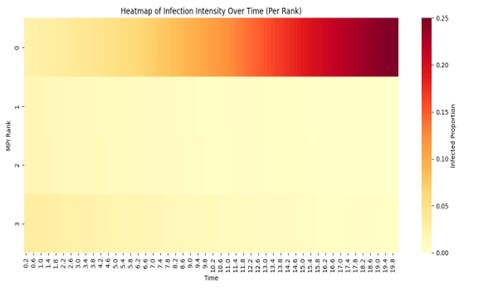
\includegraphics[width=14cm]{Images/pic2.jpg}
\end{figure}
\subsection{Performance Results and Scalability}
We compared execution time across configurations (e.g., 4 ranks, 8 ranks). As expected, total wall time decreases with more ranks, up to a limit. Communication overhead grows superlinearly due to ghost cell exchange.

\textbf{Observations}:
\begin{itemize}
    \item For 4 ranks, communication is negligible compared to computation.
    \item Communication overhead grows with process count.
    \item Load balancing is maintained via \texttt{divideIntoOptimalBlocks()}.
\end{itemize}
\begin{figure}[!htb]
    \centering
    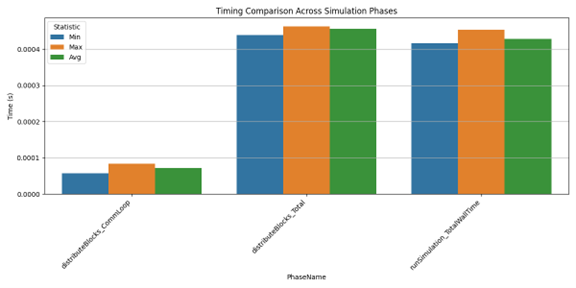
\includegraphics[width=14cm]{Images/pic4.png}
\end{figure}
\subsection{Summary of parallel implementation}
The MPI-based simulation achieves efficient spatial parallelization of the SIR model by distributing blocks of the grid across multiple processes. Each MPI rank is responsible for computing a subset of the grid, and ghost cells are exchanged between neighboring ranks to ensure correct interactions at boundaries.

This parallel structure reduces computation time significantly for large grids while preserving accuracy in local dynamics through explicit message passing. The simulation is organized in a modular fashion, separating responsibilities for grid partitioning, communication, and local updates, which improves code maintainability and profiling capabilities.
